% We discuss, how to fuse the general-purpose user-defined aggregations.
% In general, the aggregation may consume the output of more complex process.
\subsection{Background}

A reduce function processes data from a list. It has the following standard form:
\lstset{
  frame=lrtb,
  backgroundcolor=\color{white},
  numbers=left,
  numbersep=1em,
  xleftmargin=1em,
  linewidth=\linewidth
}
\begin{lstlisting}[language=code_example, caption={}]
function (:$R(I:T_1, X:\textit{List}[T_2])\rightarrow T_1$:)
  (:$s = I$:)
  foreach((:$x_i$:) in (:$X$:))
    (:$s = A(I, x_i)$:)
  return (:$F(s)$:)
\end{lstlisting}

where $I$ is the initializer , $A(s, x)$ is the user-defined accumulator, and $F(s)$ is the finalizer.
$s$ is a set of solution variables that store a partial solution,
and are initialized to the initializer $I$.
% The main foreach loop in line 3 enumerates list elements and aggregates $s$ using accumulator $A(s, x)$.
% Finally, line 4 outputs the solution according to finalizer $F$. A reduce function is then represented by the triple: $R=<I, A, F>$.
% The output $s$ of a reduce function $R$ depends on every elements of the input List $X$.

Let's consider a computational pattern shown below.
$X$, $Y$ and $Z$ are lists that have the same length. $R_1$ and $R_2$ are user-defined reduce functions.
$G$ is user-defined element-wise (broadcast is also regarded as an element-wise function) function.
There are data dependence (the producer-consumer relation) between $R_1$, $G$, and $R_2$.
They have to be executed sequentially.

\begin{lstlisting}[language=code_example, caption={Consecutive reduce functions.}]
function (:$R_1(I_1:T_1, X:\textit{List}[T_2])\rightarrow T_1$:)
  (:$s_1 = I_1$:)
  foreach((:$x_i$:) in (:$X$:)):
    (:$s_1 = A_1(I_1, x_i)$:)
  return (:$F_1(s_1)$:)

function (:$G(Z:\textit{List}[T_1])\rightarrow List[T_2]$:)  // element-wise operations
  foreach((:$z_i$:) in (:$Z$:)):
    (:$t_i = g(I_2, z_i)$:)
  return (:$T$:)  // (:\textcolor{byzantium}{$T = [\ldots, t_i, \ldots]$}:)

function (:$R_2(I_2:T_1, Y:\textit{List}[T_2])\rightarrow T_1$:)
  (:$s_2 = I_2$:)
  foreach((:$y_i$:) in (:$Y$:)):
    (:$s_1 = A_2(I_2, y_i)$:)
  return (:$F(s_2)$:)

(:$s_1 = R_1(I_1, X)$:)  // reducer 1
(:$T = G(s_1,Y,\ldots)$:)  // mapper, some element-wise function
(:$s_2 = R_2(I_2, T)$:)  // reducer 2
\end{lstlisting}

% \begin{figure}[h]
%     \centering
%     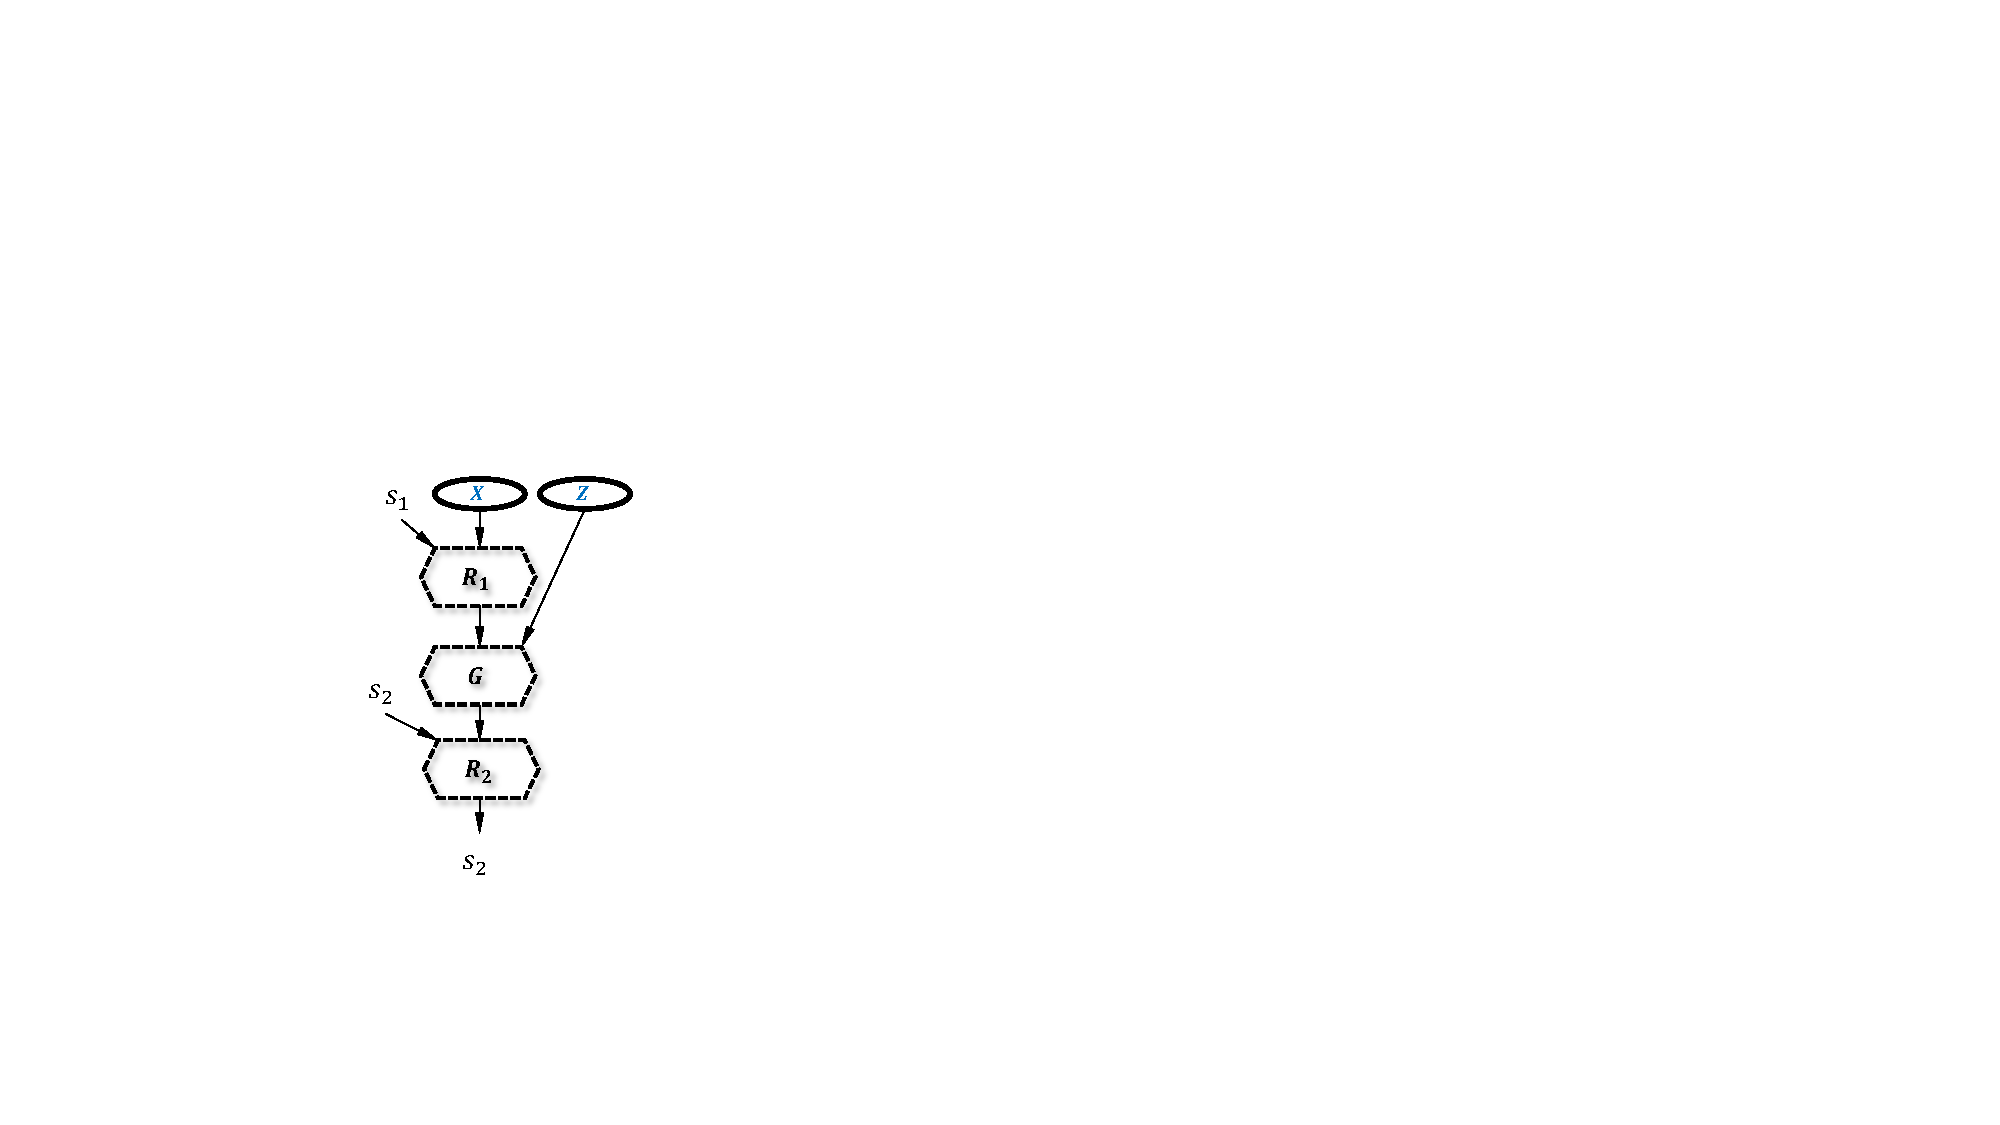
\includegraphics[width=0.2\textwidth]{figures/fuse_reduce.pdf}
%     \caption{.}
% \end{figure}

\subsection{Motivation and Goal}

In the computational pattern above, reducer $R_1$'s output $s_1$ has data dependence on each element of list $X$. Mapper $G$ consume $s_1$ and prodce a new list $T$.

reducer $R_2$'s output $s_2$ has data dependence on each element of list $T$.

The storage of $T$ might be very large.

The goal is to get a fused reduce function $s_1, s_2 = \bar{R}(I_1, I_2, s_1', s_2', X, Y)$ from $R_1$, $R_2$ and $G$.

\begin{lstlisting}[language=code_example, caption={}]
function (:$\bar{R}(p_1:T_1, p_2:T_2, I_1:T_1, I_2:T_2, X:\textit{List}[T_3],Y:\textit{List}[T_4])$:)
  (:$s_1 = I_1$:)
  (:$s_2 = I_2$:)
  foreach((:$x_i, y_1$:) in zip(:$(X, Y)$:)):
    (:$s_1',s_2' = \bar{A}(s_1, s_2, x_i, y_i, )$:) // local aggregate
    (:$s_1, s_2 = C(s_1', s_2', p_1, p_2)$:)  // combine
  return (:$s_1, s_2$:)
\end{lstlisting}

$\bar{A}$ is straightforward. It is constructed as follows:

\begin{align*}
  s_1', s_2' &= \bar{A}(I_1, I_2, s_1, s_2, x_i, y_i) \\
  s_1'&= R_1(I_1, s_1, x_i)  \\
  s_2' &= R_2(I_2, s_2, y_i)
\end{align*}

The problem is how to get $C$.
